\documentclass{beamer}

\usepackage[french]{babel}
\usepackage[utf8]{inputenc}
\usepackage[T1]{fontenc}
\usepackage{amsmath, amsthm, amsfonts}
\usepackage{siunitx}
\usepackage{tikz}
\usepackage{hyperref}
%\usepackage[backend=biber, autocite=footnote]{biblatex}
\usepackage{xcolor}
\usepackage{caption}
\usepackage{booktabs}
\usepackage{mathtools}

\tikzset{>=latex}
\usetikzlibrary{calc,decorations.pathreplacing}
\sisetup{locale=FR, per-mode=symbol}

\newcommand{\abs}[1]{\left| #1 \right|}
%\renewcommand{\vec}[1]{\ensuremath{\overrightarrow{\boldsymbol{\mathrm{ #1 }}}}}
\newcommand{\rhat}{\vec{\hat{r}}}
\newcommand{\xhat}{\vec{i}}
\newcommand{\yhat}{\vec{j}}
\newcommand{\zhat}{\vec{k}}
\newcommand{\real}{\mathbb{R}}
\newcommand{\der}[2]{\frac{\mathrm{d}#1}{\mathrm{d}#2}}
\newcommand{\pder}[2]{\frac{\partial #1}{\partial #2}}
\newcommand{\dif}{\mathrm{d}}
\newcommand{\ddif}{\,\mathrm{d}}
\newcommand{\grad}{\vec{\nabla}}
\newcommand{\exemple}[1]{\begin{fullwidth}#1\end{fullwidth}}
\newcommand{\norm}[1]{\lVert #1 \rVert}
\newcommand{\vu}{\vec{u}}
\newcommand{\vv}{\vec{v}}
\newcommand{\vr}{\vec{r}}
\newcommand{\va}{\vec{a}}
\newcommand{\vF}{\vec{F}}
\newcommand{\vecxyz}[3]{#1 \xhat + #2 \yhat + #3 \zhat}
\newcommand{\vecxy}[2]{#1 \xhat + #2 \yhat}

\theoremstyle{definition}
\newtheorem*{defn}{Definition}



\begin{document}

\begin{frame}
  \frametitle{Basketball}

  Une personne lance un ballon de basket-ball.  Au moment où celui-ci quitte
  ses mains, il est à 2 m au-dessus du sol et voyage à \SI{7.5}{m/s} selon un
  angle de \SI{55}{\degree} vers le haut par rapport à l'horizontale.  Le
  ballon pénètre dans un panier dont l'anneau est à \SI{3.05}{m} au-dessus du
  sol.  On désire calculer

  \begin{enumerate}
    \item le temps de vol du ballon
    \item la hauteur maximale du ballon par rapport au sol
    \item l'angle que forme la trajectoire du ballon avec l'horizontale lorsqu'il
          pénètre dans le panier
  \end{enumerate}

  \uncover<2>{
    \begin{center}
      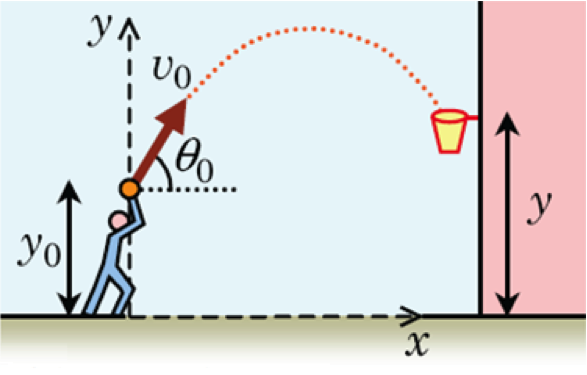
\includegraphics[scale=0.6]{basket.png}
    \end{center}
  }
\end{frame}


\begin{frame}
  \frametitle{Les pirates!}

  Un bateau pirate est muni d'un canon dont le tube forme un angle de
  \SI{30}{\degree} avec l'horizontale. Un boulet tiré par ce canon atteint un
  autre bateau situé à \SI{171}{\meter} de distance.  On désire déterminer le
  module de la vitesse initiale du boulet.

  On suppose que les bateaux sont immobiles et que la cible est à la même
  hauteur que la bouche du canon.

  \uncover<2>{
    \begin{center}
      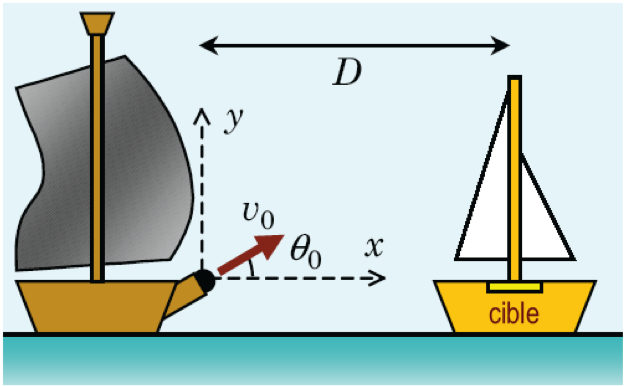
\includegraphics[scale=0.6]{pirates.png}
    \end{center}
  }
\end{frame}


\end{document}

